\mysubsection{Interface Homme $ \leftrightarrow $ Machine }

Comme point de départ du développement de l’IHM, on aura l’obtention et l’utilisation de la fonction concise obtenue en tant que produit final de l’intégration effectuée à la fin de la phase 1 (tâches 1.B.8 et 1.B.9).

Dans un premier temps, on doit définir les caractéristiques, les contraintes et  les dimensions de l’environnement de travail de l’effectuer (tableau du jeu). Alors, on doit créer les fonctions qui exécuteront les deux mouvements que le robot réalisera: “X” et “O”. Après, on doit définir les paramètres d’entrée et les données nécessaires pour le développement de l’interface et aussi la création et l’administration des objets graphiques de l’interface. Enfin, on va faire des tests, corrections nécessaires, améliorations dans l’interface et l’intégration de ses fonctionnalités avec d'autres produits finaux du projet. 

Ensuite, on a ordonné ces tâches et leurs temps estimé pour l'exécution de chaque activité:
\begin{itemize}

\item	2.B.0: Fonction concise qui détermine le paramètre d’entrée du robot (couple) à partir de la position finale et le type de trajectoire désirée (obtenue dans les tâches 1.B18 et 1.B.9): 6 créneaux; 
\item	2.B.1: Définition de les caractéristiques et dimensions d’environnement de travail (tableau du jeu): 2 créneaux;
\item	2.B.2: Définition et création de la structure de données et paramètres nécessaires pour l’IHM: 2 créneaux;
\item	2.B.3: Création des fonctions de dessin “X” et “O”: 2 créneaux;
\item	2.B.4: Définition de la disposition graphique et des objets de l’interface: 2 créneaux;
\item	2.B.5: L’insertion des éléments dans l’interface: 2 créneaux;
\item	2.B.6: Création et gestion des événements associés à les objets: 2 créneaux;
\item	2.B.7: Tests, dépannage et intégration: 3 créneaux

\end{itemize}

Ainsi, on prévoit 6 créneaux pour la réalisation de la tâche 2.B.0 qui on doit obtenir comme résultat de l’intégration des activités dans la première phase du projet et plus 15 créneaux pour l’exécution des autres tâches de cette structure.

\mysubsection{Désignation des tâches}

À partir du découpage et définition de las différentes structures du projet, on a défini que les membres Rafael Accacio et Rafael Eller seront responsables de l'exécution de la structure A du projet dans les deux phases, tandis que les membres Karoline et Tiago seront responsables de la structure B. Pour faire cette désignation des tâches, on a considéré les jours disponibles de projet (série) de chaque membre, afin que dans les jours lesquels seulement deux membres seront au laboratoire, chacun travaille en structures différentes. 	Ainsi, on prévoit obtenir une progression plus rapide et égal pour chaque structure.  

Cette organisation n’empêche pas les membres d’aider, discuter et exécuter différentes activités prévues, en prenant en compte la conclusion des tâches respectives. De plus, au fin de chaque phase on prévoit l’intégration des structures, ainsi la relation et le partage d’informations entre l’équipe sera considérée pour l’obtention de bons résultats. 

\mysubsection{Calendrier du projet}

Afin d’analyser et gérer le progrès de l’équipe et l'exécution des différentes tâches, on a fait l’estimation de la durée d’exécution des activités nécessaires pour la conclusion du projet. La table suivante décrit le calendrier de réalisation du projet: 

\begin{figure}[H]
	\begin{center}	
		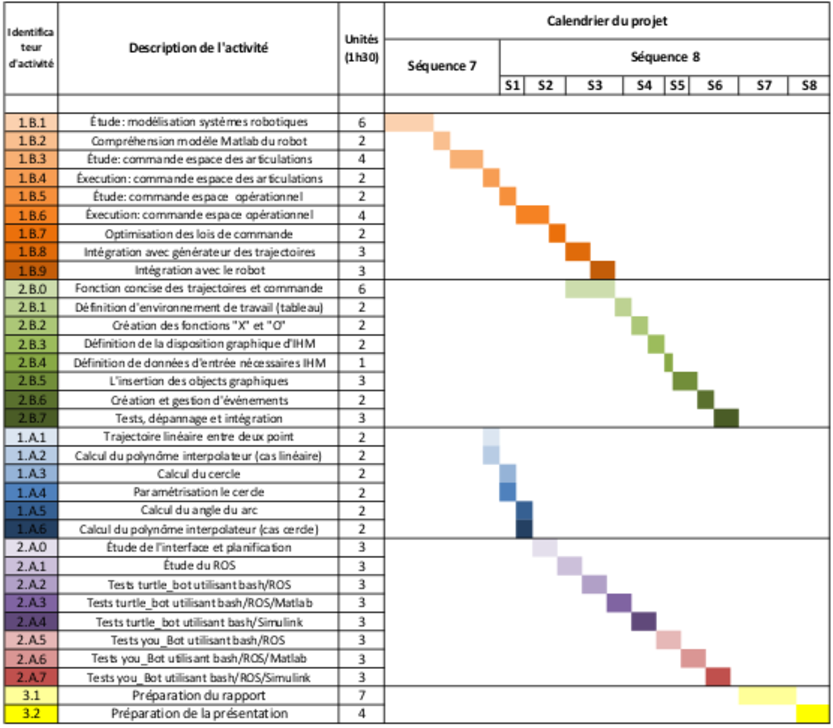
\includegraphics[width=\textwidth]{./Cronograma1}
		\caption{Calendrier de réalisation du projet.}
		\label{fig:cronograma}
	\end{center}
\end{figure}

Les unités du temps sont considérés en créneaux, dans lequel chaque créneau a 1h30 de durée. Les jours dans lesquels seulement moitié de l’équipe sera présente dans le laboratoire, on a considéré la moitié du temps de chaque créneaux. 
On aura 40 créneaux pour la séquence 8 et 54 créneaux au total pour la conclusion du projet.






